\documentclass[11pt,titlepage]{article}
%\usepackage[notref]{showkeys}
\usepackage[reqno]{amsmath}
\usepackage{natbib}
\usepackage{amssymb}
\usepackage{epsfig}
\usepackage{comment}
\usepackage{url}
\usepackage[all]{xy}        
\usepackage{dcolumn}
\newcolumntype{.}{D{.}{.}{-1}}
\newcolumntype{d}[1]{D{.}{.}{#1}}
\usepackage{threeparttable,booktabs}
\usepackage{times}
\usepackage{vmargin}
\setpapersize{USletter}
\topmargin=0in
\usepackage[compact]{titlesec}  % small
%\usepackage{ajps}
\usepackage{times}


% Shortcuts
\renewcommand{\P}{\text{P}}
\newcommand{\MC}{\multicolumn}
\usepackage{calc}
\newcounter{hours}\newcounter{minutes}
\newcommand{\printtime}{%
  \setcounter{hours}{\time/60}%
  \setcounter{minutes}{\time-\value{hours}*60}%
  \thehours :\theminutes}
%
\title{The Balance Test Fallacy in Matching Studies\thanks{Our thanks
    to Alberto Abadie, Neal Beck, Alexis Diamond, Guido Imbens, Paul
    Rosenbaum, Don Rubin, and Jas Sekhon for many helpful comments;
    and the National Institutes of Aging (P01 AG17625-01), the
    National Science Foundation (SES-0318275, IIS-9874747,
    SES-0550873), and the Princeton University Committee on Research
    in the Humanities and Social Sciences for research support.}}

\author{Kosuke Imai,\thanks{Assistant Professor, Department of
    Politics, Princeton University (Corwin Hall 041, Department of
    Politics, Princeton University, Princeton NJ 08544, USA;
    \texttt{http://Imai.Princeton.Edu}, \texttt{KImai@Princeton.Edu},
    (609) 258-6601).}
%\and %
  Gary King,\thanks{David Florence Professor of Government, Harvard
    University (Institute for Quantitative Social Science, Harvard
    University, 1737 Cambridge St., Cambridge MA 02138;
    \texttt{http://GKing.Harvard.Edu}, \texttt{King@Harvard.Edu},
    (617) 495-2027).}
%\and %
  Elizabeth A.\ Stuart\thanks{Researcher, Mathematica Policy Research,
    Inc.\, (600 Maryland Ave., SW, Suite 550, Washington, DC, 20024,
    USA; \texttt{http://people.iq.harvard.edu/$\sim$estuart/},
    \texttt{elizabeth.stuart@gmail.com}).}}

\date{\today} 

\begin{document}\maketitle
%\baselineskip=1.57\baselineskip

\begin{abstract}
  In numerous articles across a diverse variety of academic fields,
  researchers evaluate the quality of matching solutions in
  observational studies by examining $t$-tests for the difference in
  means between treatment and control groups (or sometimes via other
  hypothesis tests).  We demonstrate that this practice is fallacious
  and misleading.  We also discuss better alternatives.
\end{abstract}

Across academic fields, matching is a popular method of
nonparametrically adjusting for covariates, and reducing model
dependence, in observational studies.  Choosing one of the many
possible methods of matching

The ultimate goal of matching and the associated analyses we consider
is estimating the causal effect of a binary treatment variable $T$ on
an outcome variable $Y$.  In observational data, this typically
requires controlling for a vector of observed covariates
$X$.\footnote{Causal effects can be defined in a variety of ways,
  including average treatment effect, average treatment effect on the
  treated, etc., but the choice among these does not affect our
  argument.}  Matching is used to nonparametrically adjust the data,
by pruning or repeating observations, so that the relationship between
$X$ and $T$ --- and thus the need for subsequent parametric
adjustments for $X$ --- are eliminated or reduced.  In the best case,
the data after matching satisfy
\begin{equation}
  \label{balance}
  \tilde p(X\mid T=1) = \tilde p(X\mid T=0),
\end{equation}
where $\tilde p$ is the observed empirical density of the data, rather
than a population density.\footnote{To be more specific, the empirical
  density is defined as $\tilde p(x) = \# \{ i\in \{1, 2, \dots, n \}:
  X_i = x \} / n$, for all $x$, where $\#A$ is the number of elements
  in the set $A$.  The corresponding denominator $n$ is $\sum_{i=1}^n
  T_i$ on the left side and $\sum_{i=1}^n (1-T_i)$ on the right of
  (\ref{balance}).} In this best case, $T$ and $X$ are empirically
unrelated in the matched sample, no further adjustments for $X$ are
necessary, and the causal effect can be estimated by a simple
difference in means of $Y$ between the treatment $T=1$ and control
$T=0$ groups.  When the sample relationship between $T$ and $X$ is
reduced but not eliminated, further adjustment for $X$ may be
necessary, possibly using the same parametric methods as would have
been used if no matching had occurred \citep{HoImaKin06}.  The
immediate goal of matching, then, is to choose a matching algorithm
that satisfies (\ref{balance}) as best as possible.  Since the
methodological work on matching is growing fast, the list of available
matching algorithms is also growing.

Standard practice is for researchers to evaluate (\ref{balance}) for
each algorithm by $t$-tests for the difference in means for each
variable in $X$ between the treatment and control groups, thus
seemingly addressing at least one important aspect of a high
dimensional relationship.  Other hypothesis tests are also sometimes
used to evaluate higher dimensional diferences in (\ref{balance}), but
the same problems we describe below still applies.  The practice of
using hypothesis tests to evaluate balance is widespread, and includes
a large volume of otherwise high quality work in economics
\citep{MilFreMcH03,BlaSmi04,AgoDyn04,DehWah99, DehWah02,SmiTod05},
political science \citep{Imai05,SimHop05, Lassen05}, sociology
\citep{Harding03,DiPGan04,LunSmi05}, psychology
\citep{HavNag05,HilWalBro05,YosMagBos03,JonDAgGon04,McCRidMor04},
education \citep{Crosnoe05,SchBuc03}, management science
\citep{FreMil04, Villalonga04,WanSchAvo05}, medicine
\citep{WanSchAvo05, MacRivJur06,LinPekWan06,ManTudDie06, PetRoeMul06,
  ShiLitPot06,SabCanGib05,PerUndZho00,AusMam06,AusMamStu05}, public
health \citep{NovReaRau06,ElBGilWu05,LauSmiSta00,BinBreEar05}, and
statistics \citep{LuZanHor01}.

Tables of $t$-tests are used as a justification in published articles
for the adequacy of the chosen matching solution, and insigificant
$t$-tests are used a stopping rule during research while searching for
the right analysis to present.  This approach is problemmatic for
several reasons.  First, balance is defined for the sample, not some
hypothetical population, and so strictly speaking hypothesis tests are
irrelevant.  For the same reason that randomized blocks are preferable
to classical randomization in experimental design, matching as well as
possible on all observables is preferable.  

Second, the smaller the difference between $\tilde p(X\mid T=1)$
$\tilde p(X\mid T=0)$, the better, and this is true without limit.
Matching contains no de minimus standard, below which the level of
imbalance is acceptable.  Suppose, for example, the data are generated
by the classical regression model, $E(Y)= \theta + T\beta + X\gamma$.
Then the regression of $Y$ on a constant and $T$ gives a difference in
means, the bias of which is $E(\hat\beta) = F\gamma$, where $F$ are
the coefficients of regressions of variables in $X$ on $T$.  Matching,
under this simplified data generation process, seeks to eliminate the
bias by dropping observations in order to make $F$ as close to a
vector of zeros as possible.  But what happens to bias if $F$ is
smaller than it was before matching but still not zero?  It gets
smaller, but without knowledge of $\gamma$ --- which matching
researchers eschew estimating to ensure that they do not inadvertently
choose matching solutions in order to favor their favored hypotheses
--- it could be that the nonzero portion of $F$ could generate
arbitrarily large bias.

Since the estimation bias of the causal
effect is a function of imbalance and also the effect of $X$ on $Y$
given $T$, any difference between the control and treatment groups can
produce biases of any size.




To illustrate the problem we pose, consider a data set where $Y$ is
..., $T$ is ..., and $X$ includes ....  These data include a large
pool of potential control ($T=0$) units.  Matching begins with the
full data set and then selectively deletes observations until
(\ref{balance}) is best satisfied without losing too many
observations.  Suppose however that our matching algorithm had no
effect on bias; suppose in fact it involved entirely random selection
of observations to discard.  Clearly, this algorithm would not effect
balance, or the bias in the ultimate analysis that satisfying
(\ref{balance}) is meant to achieve.  Yet, we can show that randomly
deleting observations does wonders according to the $t$-test.  To do
this, we create a sequence of matching solutions that randomly drop
different numbers of control observations.  

The left graph in Figure \ref{f:randrop} presents the results.  The
horizontal axis in this figure reports the number of control units
randomly dropped, while the vertical axis gives the size of the
$t$-test.  We have shaded in the area below a $t$-test of 2, the
conventional threshold for statistical insignificance and the usual
goal of these tests.  The line on the plot clearly shows that
according to the $t$-test, randomly dropping more control units does
an ``excellent'' job at achieving balance, which of course makes no
sense at all.
\begin{figure}[t]
  \centering
  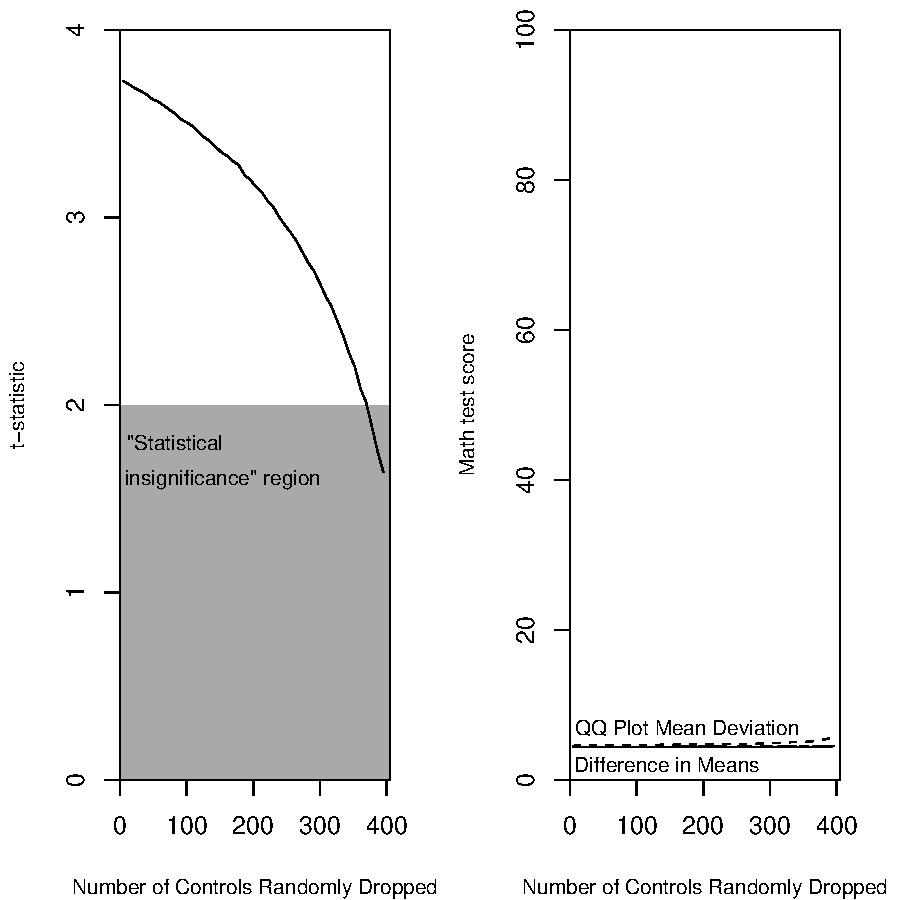
\includegraphics[height=4.5in]{figs/TStatPlotR0MATH}
  \caption{Dangers in relying on $t$-statistics as measure of balance.
    The solid lines in both graphs indicate the average value of a
    measure of balance when a given number of control units are
    randomly dropped from the data set (out of a total of ***).  With
    larger numbers of control units dropped (i.e., smaller numbers of
    control units in the resulting sample), the t-statistic gets
    closer to 0, falsely indicating improvements in balance with the
    smaller resulting sample sizes, even though true balance does not
    vary systematically across the data sets (and efficiency
    declines).  The difference in means and QQ plot mean deviation,
    given in the right graph, correctly indicate no change in bias as
    observations are randomly dropped.}
  \label{f:randrop}
\end{figure}

The problem is that dropping observations can influence not only
balance but also statistical power.  The more observations dropped,
the less power the tests have to detect problems.  More formally, we
can write the two sample $t$-test statistic (TS) with unknown and
unequal variances as
\begin{equation}
  \label{ttest}
\text{(TS)} = \frac{\sqrt{n}(\overline{X}_t-\overline{X}_c)}
               {\sqrt{\frac{s^2_t}{r} + \frac{s^2_c}{1-r}}}
\end{equation}
where $s^2_t=\sum_{i=1}^n t_i(X_i - \overline{X}_t)^2/(n_t-1)$,
$s^2_c=\sum_{i=1}^n (1-t_i)(X_i - \overline{X}_t)^2/(n_c-1)$, $n_t$
and $n_c$ are the sample sizes for the treatment and control groups,
respectively, and $r=n_t/n$.  Hence, the difference in sample means as
a measure of balance is distorted in the $t$-test by three factors:
(1) the total number of remaining observations $n$, (2) the ratio of
remaining treated units to the total number of remaining observations
$r$, and (3) the variance of $X$ for the remaining treated and control
units, $s_t^2$ and $s_c^2$.  Since the value of (this and other)
hypothesis tests are affected by factors other than balance, they
cannot even be counted on to be monotonic functions of balance: The
$t$-test can indicate balance is getting better while the actual
balance is getting worse, staying the same, or improving.

2 views:

1. everything in subsequent analyses is conditional on X, in
sample. and so hypothetical populations are irreelvant.  any sampling
process on X is irrelevant.

2. suppose there is measurement error in X but not T.  observe sample
of areal units and want to match on those units.  i.e., tests are ok
if there is known uncertainty.  in this situation, we would need a
test rather than observed matches, but such a test has not been
proposed.  present t-test doesn 't help in this situation, but further
research might produce something for which power is not a function of
the remaining sample size.  open question: could we balance better if
we knew we had random measurement error than conditioning on the
observed value?

imagine 2 possible experiments:  one is matched pairs plus random toss
for t.  the other is random assignment between treatment and control
groups.  

alternatives: general point is to compare 2 multidimensional
histograms. raw diff in means, variances and other statitics.  qq
plots are excellent general procedures.  see right graph in figure 2.


%\baselineskip=0.637\baselineskip 
\bibliographystyle{apsr}
\bibliography{gk,gkpubs}

\end{document}
